\section{Setup} 
I'm using my own computer with Ubuntu 18.04, Visual Studio Code and Cmake to complete the labs.

\section{Introduction to 2D Computer Graphics}

\subsection{Color the screen}
I experimented with the color model by setting the color to 
\begin{enumerate}
    \item red: \texttt{vec3 color(1, 0, 0)}
    \item green: \texttt{vec3 color(0, 1, 0)}
    \item blue: \texttt{vec3 color(0, 0, 1)}
    \item yellow: \texttt{vec3 color(1, 1, 0)}
    \item magenta: \texttt{vec3 color(1, 0, 1)}
    \item black: \texttt{vec3 color(0, 0, 0)}
    \item white: \texttt{vec3 color(1, 1, 1)}
\end{enumerate}

\subsection{Linear Interpolation}
I wrote the function \texttt{void Interpolate( float a, float b, vector<float>\& result );} using the formula for linear interpolation:
To interpolate between two points \(x_0\) and \(x_1\) we use
\begin{equation}\label{eq:lin_inter}
    f(x)=\frac{x_1-x}{x_1-x_0}f(x_0)+\frac{x-x_0}{x_1-x_0}f(x_1)
\end{equation}
The range of \texttt{x} is given by the size of the result vector: \(x \in [0, result.size()-1]\).\\
To catch the special cases if the result vector has size 0 or 1 I return immediately if the size is 0 and I return the average of \texttt{a} and \texttt{b} in
case the size is 1. Otherwise I use equation (\refeq{eq:lin_inter}).\\
I tested my implementation with the values and output given in the assignment instructions. To do that I wrote the function \texttt{void TestFloatInterpolate()}.\\
To implement \texttt{void Interpolate(glm::vec3 a, glm::vec3 b, std::vector<glm::vec3>\& result)} I used the same approach and applied it to each dimension of the 
\texttt{vec3}.
I tested my implementation with the values and output given in the assignment instructions. To do that I wrote the function \texttt{void TestVec3Interpolate()}.
\newpage
\subsection{Bilinear Interpolation of Colors}
\texttt{glm::vec3 topLeft(1,0,0); // red \\
glm::vec3 topRight(0,0,1); // blue\\
glm::vec3 bottomLeft(1,1,0); // yellow\\
glm::vec3 bottomRight(0,1,0); // green }
\begin{figure}[ht]
        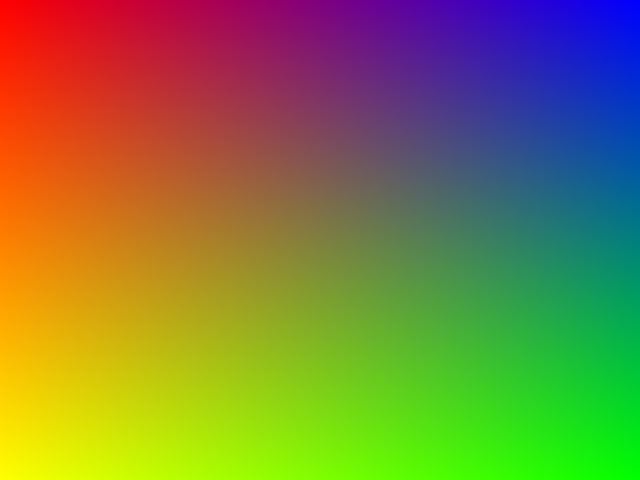
\includegraphics[width=10cm]{screenshots/bil_inter_1.png}
\end{figure}
\\
% \clearpage
\texttt{glm::vec3 topLeft(1,0,1); // magenta\\
	glm::vec3 topRight(1,1,1); // white\\
	glm::vec3 bottomLeft(0,1,1); // cyan\\
	glm::vec3 bottomRight(0,0,0); // black}
\begin{figure}[ht]
        
\includegraphics[width=10cm]{screenshots/bil_inter_2.png}
\end{figure}

\section{Starfield}
\subsection{Static Starfield}
To create a static starfield in \texttt{main} I first initialize all star positions randomly in the given range. Then I project the x and y positions with the
equations of the pinhole camera.\\
\begin{figure}[ht]
    \begin{center}
        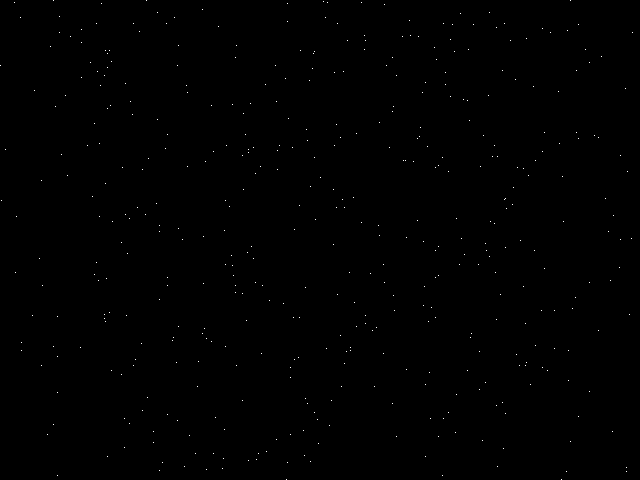
\includegraphics[width=10cm]{screenshots/static_starfield.png}
        \caption{static starfield}
    \end{center}
\end{figure}
\\
The viewing angle can be calculated with equation \eqref{eq:viewing_angle}:
\begin{equation}\label{eq:viewing_angle}
    tan(\frac{\alpha}{2})=\frac{L}{2f}
\end{equation}
where \texttt{f} is the focal length and \texttt{L} is the length of the image. So if we use \(f=H/2\) and want to compute the horizontal field of view we get
\(tan(\frac{\alpha}{2})=\frac{W}{2f}\) where W is the screen width. We use H=480 and W=640. If we calculate we get \(\alpha=106.26\degree\).

\subsection{Motion}
To create the motion effect in the \texttt{Upddat()} function I update each star's distance value with \\
\texttt{stars[s].z -= VELOCITY * dt / 1000.0f; //use dt in seconds, velocity is in m/s}. \\
\texttt{dt} is in milliseconds, therefore I divide by 1000.0f so 
that I can choose the velocity in \texttt{m/s}. For the velocity I chose a value of 5. With that I get a reasonable moving starfield effect.